% Options for packages loaded elsewhere
\PassOptionsToPackage{unicode}{hyperref}
\PassOptionsToPackage{hyphens}{url}
%
\documentclass[
  ignorenonframetext,
  aspectratio=1610,
]{beamer}
\usepackage{pgfpages}
\setbeamertemplate{caption}[numbered]
\setbeamertemplate{caption label separator}{: }
\setbeamercolor{caption name}{fg=normal text.fg}
\beamertemplatenavigationsymbolsempty
% Prevent slide breaks in the middle of a paragraph
\widowpenalties 1 10000
\raggedbottom
\setbeamertemplate{part page}{
  \centering
  \begin{beamercolorbox}[sep=16pt,center]{part title}
    \usebeamerfont{part title}\insertpart\par
  \end{beamercolorbox}
}
\setbeamertemplate{section page}{
  \centering
  \begin{beamercolorbox}[sep=12pt,center]{part title}
    \usebeamerfont{section title}\insertsection\par
  \end{beamercolorbox}
}
\setbeamertemplate{subsection page}{
  \centering
  \begin{beamercolorbox}[sep=8pt,center]{part title}
    \usebeamerfont{subsection title}\insertsubsection\par
  \end{beamercolorbox}
}
\AtBeginPart{
  \frame{\partpage}
}
\AtBeginSection{
  \ifbibliography
  \else
    \frame{\sectionpage}
  \fi
}
\AtBeginSubsection{
  \frame{\subsectionpage}
}
\usepackage{amsmath,amssymb}
\usepackage{iftex}
\ifPDFTeX
  \usepackage[T1]{fontenc}
  \usepackage[utf8]{inputenc}
  \usepackage{textcomp} % provide euro and other symbols
\else % if luatex or xetex
  \usepackage{unicode-math} % this also loads fontspec
  \defaultfontfeatures{Scale=MatchLowercase}
  \defaultfontfeatures[\rmfamily]{Ligatures=TeX,Scale=1}
\fi
\usepackage{lmodern}
\ifPDFTeX\else
  % xetex/luatex font selection
\fi
% Use upquote if available, for straight quotes in verbatim environments
\IfFileExists{upquote.sty}{\usepackage{upquote}}{}
\IfFileExists{microtype.sty}{% use microtype if available
  \usepackage[]{microtype}
  \UseMicrotypeSet[protrusion]{basicmath} % disable protrusion for tt fonts
}{}
\makeatletter
\@ifundefined{KOMAClassName}{% if non-KOMA class
  \IfFileExists{parskip.sty}{%
    \usepackage{parskip}
  }{% else
    \setlength{\parindent}{0pt}
    \setlength{\parskip}{6pt plus 2pt minus 1pt}}
}{% if KOMA class
  \KOMAoptions{parskip=half}}
\makeatother
\usepackage{xcolor}
\newif\ifbibliography
\usepackage{longtable,booktabs,array}
\usepackage{calc} % for calculating minipage widths
\usepackage{caption}
% Make caption package work with longtable
\makeatletter
\def\fnum@table{\tablename~\thetable}
\makeatother
\usepackage{graphicx}
\makeatletter
\def\maxwidth{\ifdim\Gin@nat@width>\linewidth\linewidth\else\Gin@nat@width\fi}
\def\maxheight{\ifdim\Gin@nat@height>\textheight\textheight\else\Gin@nat@height\fi}
\makeatother
% Scale images if necessary, so that they will not overflow the page
% margins by default, and it is still possible to overwrite the defaults
% using explicit options in \includegraphics[width, height, ...]{}
\setkeys{Gin}{width=\maxwidth,height=\maxheight,keepaspectratio}
% Set default figure placement to htbp
\makeatletter
\def\fps@figure{htbp}
\makeatother
\setlength{\emergencystretch}{3em} % prevent overfull lines
\providecommand{\tightlist}{%
  \setlength{\itemsep}{0pt}\setlength{\parskip}{0pt}}
\setcounter{secnumdepth}{-\maxdimen} % remove section numbering
\ifLuaTeX
\usepackage[bidi=basic]{babel}
\else
\usepackage[bidi=default]{babel}
\fi
\babelprovide[main,import]{english}
% get rid of language-specific shorthands (see #6817):
\let\LanguageShortHands\languageshorthands
\def\languageshorthands#1{}
\usepackage{pgfpages}
\usepackage{microtype}
\usepackage{tikz}
  \usetikzlibrary{positioning}
  \usetikzlibrary{arrows}
  \usetikzlibrary{graphs}

\definecolor{CTred}{RGB}{229,32,32}
\definecolor{CTgrey}{RGB}{153,153,153}

\usepackage{array}
\usepackage{dcolumn}
\newcolumntype{d}{D{.}{.}{-1}}
\usepackage{booktabs}
\usepackage{threeparttable}

% colors: white text on 90% black background
\setbeamercolor{normal text}{fg=black,bg=white}

% light blue as a highlight color
\setbeamercolor*{structure}{fg=CTred}
\setbeamercolor{section title}{fg=CTred}
\setbeamercolor{alerted text}{use=structure,fg=CTred}
\setbeamercolor*{palette primary}{use=structure,fg=structure.fg}
\setbeamercolor*{palette secondary}{use=structure,fg=structure.fg!95!black}
\setbeamercolor*{palette tertiary}{use=structure,fg=structure.fg!90!black}
\setbeamercolor*{palette quaternary}{use=structure,fg=structure.fg!95!black,bg=black!80}

\setbeamercolor*{framesubtitle}{fg=white}


% use system fonts: here, Gill Sans
\usefonttheme{professionalfonts}
\setbeamerfont{quote}{shape=\upshape}

% eliminate silly beamer navigation line at bottom of slides
\setbeamertemplate{navigation symbols}{}
\setbeamertemplate{footline}[frame number]

% ensure text jusfication
\usepackage{ragged2e}
\justifying

% pandoc makes 2nd-lever headers into blocks, and this ensures justification
% in blocks too
\addtobeamertemplate{block begin}{}{\justifying}




\urlstyle{same}
\usepackage[overlay,absolute]{textpos}

\setbeamertemplate{items}[square]

\TPGrid[10 mm,8 mm]{9}{8}
% beamer's left and right margin is 10 mm. The top/bottom margin is ??
% or without a header ??
% the slide dimensions are 128 mm x 96 mm
% so the resulting \TPHorizModule = 12 mm and \TPVertModule = 10 mm

% uncomment if you want biblatex for citations on slides

% \usepackage{csquotes}
% \usepackage[notes,short,noibid,backend=biber]{biblatex-chicago}
% \bibliography{course.bib} 

\providecommand{\exhibit}[2]{\includegraphics[keepaspectratio, height=0.9\textheight, width=\textwidth]{assets/img/#1}\\ {\tiny #2}}

\providecommand{\smallcite}[1]{({\footnotesize #1})}
\ifLuaTeX
  \usepackage{selnolig}  % disable illegal ligatures
\fi
\IfFileExists{bookmark.sty}{\usepackage{bookmark}}{\usepackage{hyperref}}
\IfFileExists{xurl.sty}{\usepackage{xurl}}{} % add URL line breaks if available
\urlstyle{same}
\hypersetup{
  pdftitle={Sudden Liberalization and the Baby Boom of Managers},
  pdfauthor={Miklós Koren; Krisztina Orbán},
  pdflang={en},
  hidelinks,
  pdfcreator={LaTeX via pandoc}}

\title{Sudden Liberalization and the Baby Boom of Managers}
\author{Miklós Koren \and Krisztina Orbán}
\date{June 2, 2023}

\begin{document}
\frame{\titlepage}
\begin{abstract}
Good management practices are important determinants of firm success.
Better managed firms are larger and more productive, and management
interventions lead to sizeable and persistent positive effects on firm
performance. It is unclear, however, to what extent aggregate outcomes
are shaped by good management. We build an overlapping generations model
of managers to study the demand and supply of good management and the
competition between managers of heterogeneous skills. We use data on the
universe of corporations and their top managers in Hungary between 1985
and 2019 to study the rapid liberalization of the 1990s through the lens
of our model. We use the model to evaluate hypothetical policies aiming
to improve aggregate productivity through management education and
corporate liberalization. Our results suggest that the inelastic supply
of good managers is an important constraint to the success of management
interventions.
\end{abstract}

\hypertarget{introduction}{%
\section{Introduction}\label{introduction}}

\begin{frame}{Research Question}
\protect\hypertarget{research-question}{}
\begin{enumerate}
\tightlist
\item
  How elastic is the supply of good management?
\item
  What are the consequences for aggregate outcomes of a potential low
  elasticity?
\item
  How long-lasting are the aggregate effects of the low elasticity?
\end{enumerate}
\end{frame}

\begin{frame}{Why Supply Matters}
\protect\hypertarget{why-supply-matters}{}
\begin{block}{The McKinsey view}
\protect\hypertarget{the-mckinsey-view}{}
Everyone can be a good manager after paying \$\$\$. If demand for
management goes up, all firms become better.
\end{block}

\begin{block}{Inelastic supply}
\protect\hypertarget{inelastic-supply}{}
There is a fixed number of good managers. If demand for management goes
up, good managers earn more.
\end{block}
\end{frame}

\begin{frame}{But Can Management Increase Aggregate GDP?}
\protect\hypertarget{but-can-management-increase-aggregate-gdp}{}
We don't know:

\begin{enumerate}
\tightlist
\item
  How elastic is the aggregate supply of good managers?
\item
  What role for equilibrium feedback?
\end{enumerate}
\end{frame}

\begin{frame}{Literature}
\protect\hypertarget{literature}{}
\begin{enumerate}
\tightlist
\item
  \textbf{Management as technology}: Bloom et al (2010), Bertrand and
  Schoar (2003), Bloom et al (2013), Giorcelli (2019)

  \begin{itemize}
  \tightlist
  \item
    This paper: Acknowledging that often these interventions are very
    hard to scale, what are the aggregate implications of heterogeneity
    in management?
  \end{itemize}
\item
  \textbf{Firm heterogeneity at entry along the business cycle}:
  Sedlaček and Sterk (2018)

  \begin{itemize}
  \tightlist
  \item
    This paper: What is the role of manager selection in this firm
    selection?
  \end{itemize}
\item
  \textbf{Consequences of lack of delegation in family firms for
  development}: Caselli, Gennaioli (2013), Akcigit, Alp, Peters (2021)

  \begin{itemize}
  \tightlist
  \item
    This paper: Dynamics and anatomy of adjustment via managers to a
    demand increase
  \end{itemize}
\end{enumerate}
\end{frame}

\begin{frame}{This paper}
\protect\hypertarget{this-paper}{}
\begin{enumerate}
\tightlist
\item
  Assemble a dataset on the universe of managers in the Hungarian
  economy (1985 -- 2021) + firm balance sheet info
\item
  Examine a large liberalization episode in Hungary in which the demand
  for management skills increased 20-fold
\item
  Build an OLG model of managers with heterogeneous manager skills to
  capture:

  \begin{itemize}
  \tightlist
  \item
    Existing manager stock in an economy is an important determinant of
    current manager entry
  \item
    Large existing competition reduces current entry to an inefficient
    extent
  \item
    Friction to occupational switching cause this reduced entry to have
    long-term consequences on aggregates
  \end{itemize}
\item
  Model will be used for counterfactuals: effect of education reform,
  effect of spacing out liberalization's effect on manager entry.
\end{enumerate}
\end{frame}

\begin{frame}{Outline}
\protect\hypertarget{outline}{}
\begin{enumerate}
\tightlist
\item
  Setup and data
\item
  An OLG model of managers
\item
  A numerical example for policy analysis
\item
  Facts about Hungarian corporations and their CEOs, 1988-2019
\end{enumerate}
\end{frame}

\hypertarget{data}{%
\section{Data}\label{data}}

\begin{frame}{Manager Data 1988-2019}
\protect\hypertarget{manager-data-1988-2019}{}
\begin{block}{Manager}
\protect\hypertarget{manager}{}
Top officer of corporation (CEO). 1m corporations, 1.3m CEOs.

No socioeconomic or demographic information, only identifiers. Sometimes
age, can infer gender and nationality (not today).
\end{block}

\begin{block}{Worker}
\protect\hypertarget{worker}{}
10\% sample of workforce. Repeated cross section. All managerial
occupations, including middle management.
\end{block}
\end{frame}

\begin{frame}{Financials}
\protect\hypertarget{financials}{}
\begin{itemize}
\tightlist
\item
  Annual panel of balance sheets and earning statements of corporations
  with double-entry bookkeeping. 936k firms, 8.4m observations.
\item
  Use sales inflated to 2019, employment, and 2-digit NACE sector.
\end{itemize}
\end{frame}

\begin{frame}{The Stock of Managers Increased Sharply Relative to 35-60
Age Group}
\protect\hypertarget{the-stock-of-managers-increased-sharply-relative-to-35-60-age-group}{}
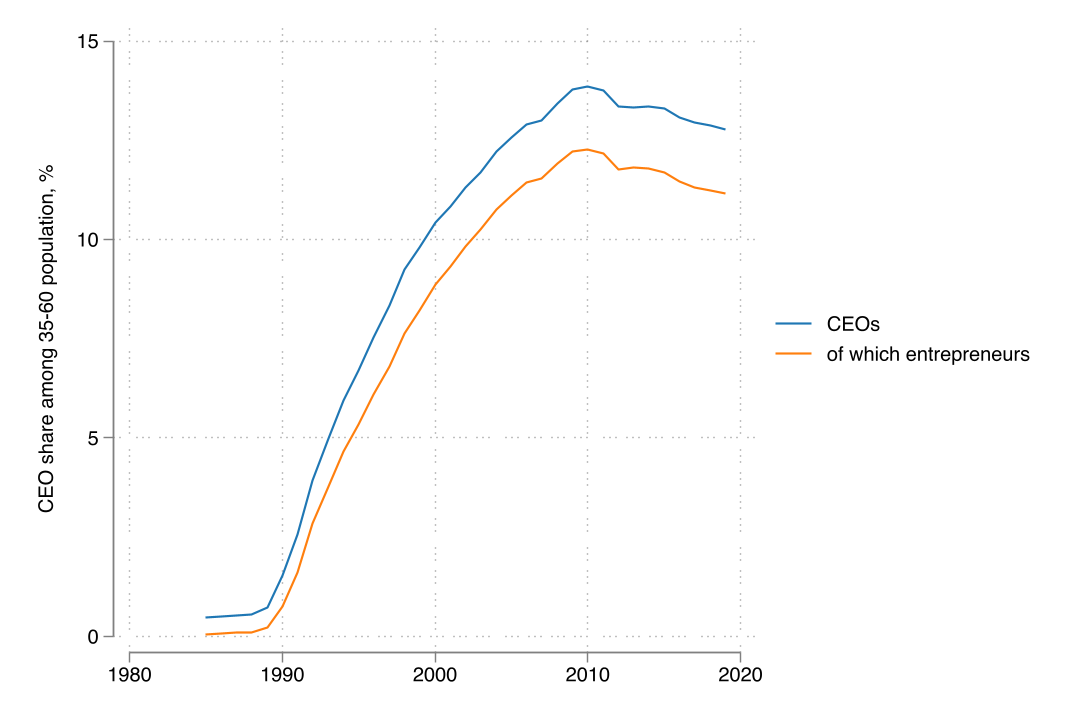
\includegraphics{fig/ceo-stock.png}
\end{frame}

\begin{frame}{Managerial Jobs Increased in Both Quantity and Price}
\protect\hypertarget{managerial-jobs-increased-in-both-quantity-and-price}{}
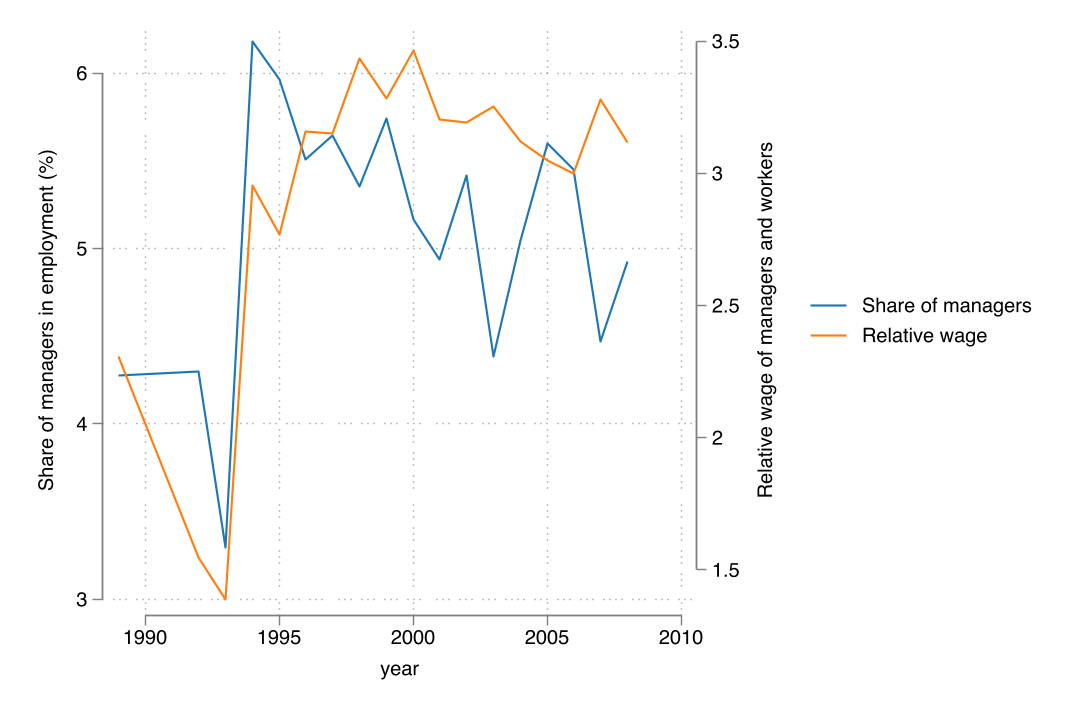
\includegraphics{fig/fixed/age-relative-wage.png}
\end{frame}

\hypertarget{an-olg-model-of-managers}{%
\section{An OLG Model of Managers}\label{an-olg-model-of-managers}}

\begin{frame}{An OLG Model of Managers}
\protect\hypertarget{an-olg-model-of-managers-1}{}
An overlapping generations model with heterogeneous manager skill,
limited span of control and career choice. Each time \(t\), \(l\)
individuals are born. Only \(n(t) < l\) choose to become managers. They
remain a manager until they die.

\begin{block}{Key decision}
\protect\hypertarget{key-decision}{}
career choice
\end{block}

\begin{block}{Key equilibrium feedback}
\protect\hypertarget{key-equilibrium-feedback}{}
competition across cohorts
\end{block}

\begin{block}{Key friction}
\protect\hypertarget{key-friction}{}
managers cannot switch out of their choice to become managers
\end{block}
\end{frame}

\begin{frame}{Production Function}
\protect\hypertarget{production-function}{}
Managers differ in their innate skill level. A manager with skill \(z\)
can hire \(h\) workers to produce output with the production function
\[q = z^\nu h^{1-\nu}\] \(\nu>0\) captures span of control (Lucas 1978):
hard to run a large firm.
\end{frame}

\begin{frame}{Competition Between Managers}
\protect\hypertarget{competition-between-managers}{}
Potential new managers have a time invariant skill distribution
\(F(z)\).

Only the best become managers: a time varying truncation of \(F\).

The distribution of skill among the stock of managers, denoted by
\(G(t, z)\), is a mixture of these truncated distributions.
\end{frame}

\begin{frame}{Dynamics}
\protect\hypertarget{dynamics}{}
The change in the overall skill of managers is a slowly moving state
variable. \[Z'(t) = n(t)\tilde z(t) - \delta Z(t)\]

Bellman equation for manager value:
\[\rho v(t) = \nu p \left[\frac {L^{p}(t)}{Z(t)}\right]^{1-\nu} - \delta v(t) + v'(t)\]
\end{frame}

\begin{frame}{Career Choice}
\protect\hypertarget{career-choice}{}
Potential managers choose to enter if value exceeds exogenous cost
\(\tau\) and the opportunity cost, \[v(t)z > (1+\tau)J(t)\]

Selection on manager skill, \(z > \frac {(1+\tau)J(t)} {v(t)}\).
\end{frame}

\begin{frame}{Predictions}
\protect\hypertarget{predictions}{}
The steady-state stock of manager skills \emph{and GDP} are increasing
in:

\begin{enumerate}
\tightlist
\item
  Number of workers
\item
  Manager elasticity \(\nu\) and prices
\item
  The location shifter of manager skill distribution.
\end{enumerate}

They are decreasing in:

\begin{enumerate}
\tightlist
\item
  Discount rate and death rate
\item
  Costs of doing business.
\end{enumerate}
\end{frame}

\begin{frame}{Transitional Dynamics}
\protect\hypertarget{transitional-dynamics}{}
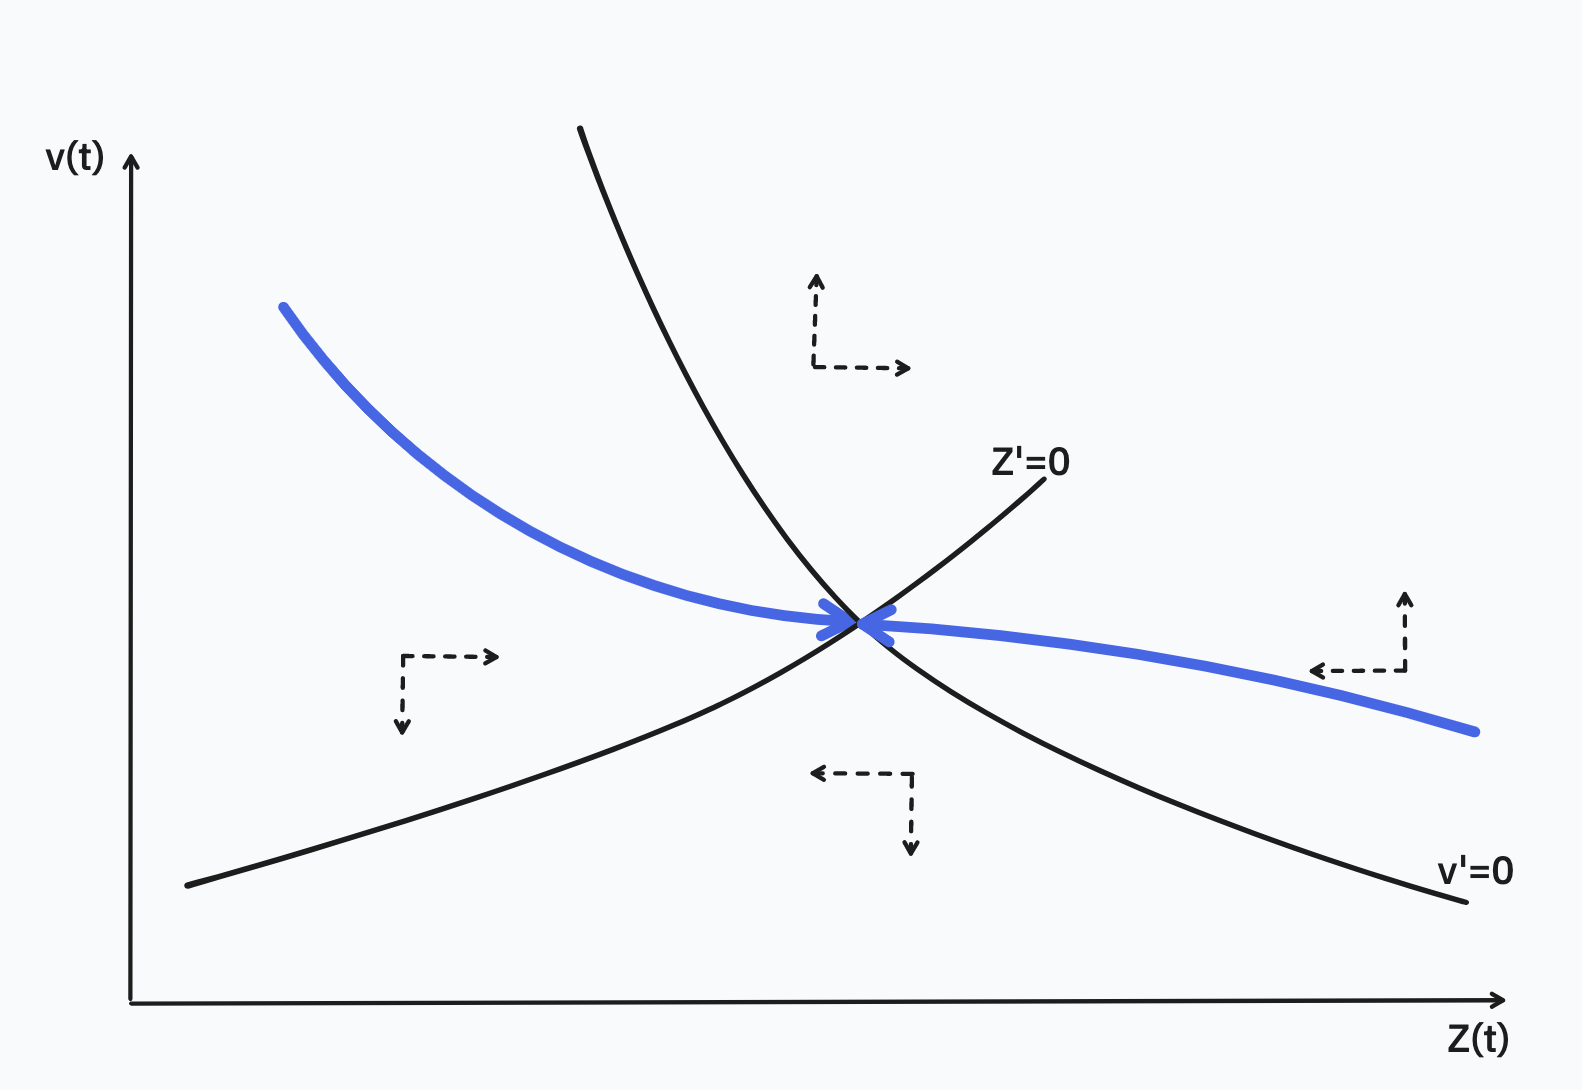
\includegraphics{fig/phase1.png}
\end{frame}

\hypertarget{taking-the-model-to-the-data}{%
\section{Taking the Model to the
Data}\label{taking-the-model-to-the-data}}

\begin{frame}{Calibration}
\protect\hypertarget{calibration}{}
\begin{longtable}[]{@{}
  >{\raggedright\arraybackslash}p{(\columnwidth - 6\tabcolsep) * \real{0.2500}}
  >{\raggedright\arraybackslash}p{(\columnwidth - 6\tabcolsep) * \real{0.2500}}
  >{\raggedright\arraybackslash}p{(\columnwidth - 6\tabcolsep) * \real{0.2500}}
  >{\raggedright\arraybackslash}p{(\columnwidth - 6\tabcolsep) * \real{0.2500}}@{}}
\toprule\noalign{}
\begin{minipage}[b]{\linewidth}\raggedright
Parameter
\end{minipage} & \begin{minipage}[b]{\linewidth}\raggedright
Value
\end{minipage} & \begin{minipage}[b]{\linewidth}\raggedright
Meaning
\end{minipage} & \begin{minipage}[b]{\linewidth}\raggedright
Target
\end{minipage} \\
\midrule\noalign{}
\endhead
\bottomrule\noalign{}
\endlastfoot
\(\nu\) & \(0.15\) & Manager elasticity & Income share of managers \\
\(\theta\) & \(1.5\) & Skill heterogeneity & Wage premium of managers \\
\(\tau\) & \(2\) & Cost of doing business & Suppressed income share of
managers \\
\(\delta\) & \(0.033\) & Exit rate of managers & Manager life cycle \\
\end{longtable}
\end{frame}

\begin{frame}{Alternative calibrations (todo)}
\protect\hypertarget{alternative-calibrations-todo}{}
\begin{block}{No skill heterogeneity}
\protect\hypertarget{no-skill-heterogeneity}{}
\(\theta\to\infty\) so that average = marginal manager
\end{block}

\begin{block}{Immediate response}
\protect\hypertarget{immediate-response}{}
\(\delta\to\infty\) so that manager turnaround is quick
\end{block}
\end{frame}

\hypertarget{policy-counterfactuals}{%
\section{Policy Counterfactuals}\label{policy-counterfactuals}}

\begin{frame}{Sudden liberalization}
\protect\hypertarget{sudden-liberalization}{}
Transition from communism to capitalism, leading to a drastic fall in
\(\tau\).
\end{frame}

\begin{frame}{Sudden Liberalization}
\protect\hypertarget{sudden-liberalization-1}{}
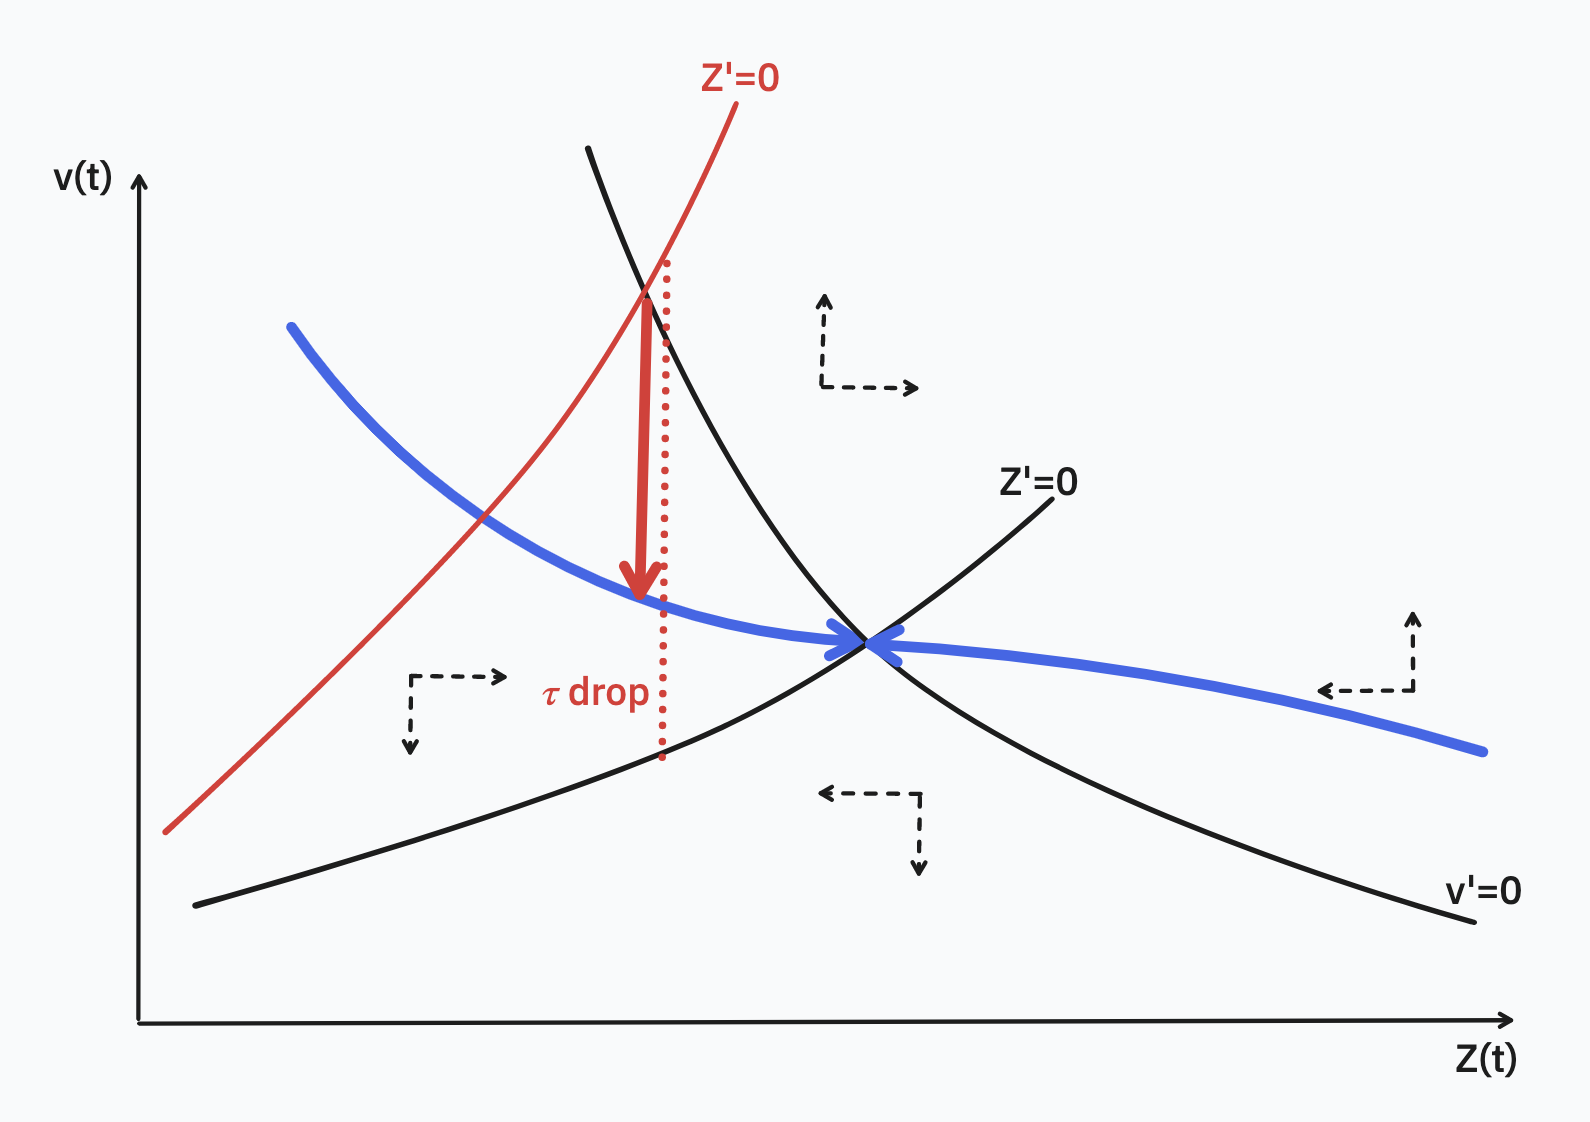
\includegraphics{fig/phase2.png}
\end{frame}

\begin{frame}{Entry Jumps Then Gradually Declines}
\protect\hypertarget{entry-jumps-then-gradually-declines}{}
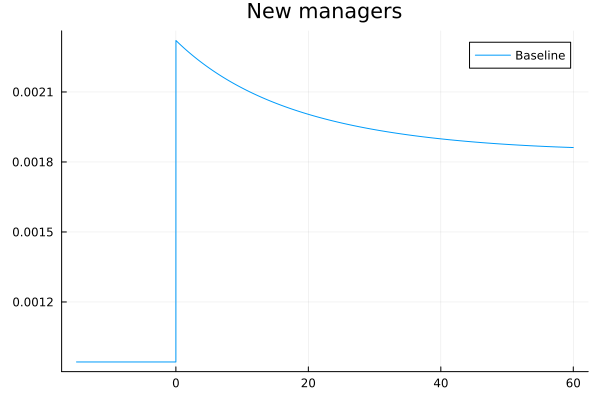
\includegraphics{fig/model-entry-liberalization.png}
\end{frame}

\begin{frame}{GDP Slowly Converges to New Steady State}
\protect\hypertarget{gdp-slowly-converges-to-new-steady-state}{}
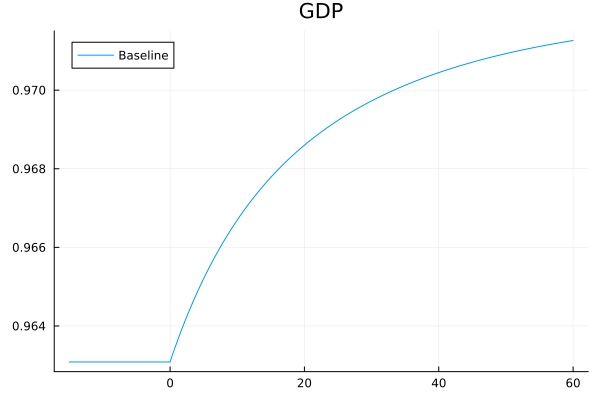
\includegraphics{fig/model-gdp-liberalization.png}
\end{frame}

\begin{frame}{Entrant Skill Drops Sharply}
\protect\hypertarget{entrant-skill-drops-sharply}{}
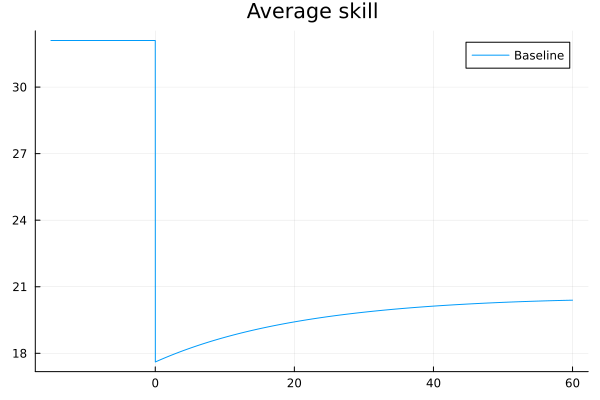
\includegraphics{fig/model-skill-liberalization.png}
\end{frame}

\hypertarget{conclusion}{%
\section{Conclusion}\label{conclusion}}

\begin{frame}{Conclusion}
\protect\hypertarget{conclusion-1}{}
\begin{itemize}
\tightlist
\item
  OLG model with manager heterogeneity, featuring inefficient entry of
  managers in response to demand shock, with long run consequences for
  aggregates
\item
  Slow response to sudden liberalization.
\item
  New cohort of managers has lower skill levels.
\end{itemize}
\end{frame}

\begin{frame}{Next Steps}
\protect\hypertarget{next-steps}{}
\begin{itemize}
\tightlist
\item
  Track distribution of manager skills, not just Z, allows exit by worst
  managers
\item
  Allow old generation to build customer capital
\item
  Allow managers' skill to evolve over time
\item
  Separate firm and manager, allow firm heterogeneity
\end{itemize}
\end{frame}

\end{document}
